\documentclass[../main/main.tex]{subfiles}

\newdate{date}{28}{10}{2020}

% \begin{figure}[h!]
% \centering
% \includegraphics[page=6,width=0.8\textwidth]{../lessons/pdf_file/12_lecture.pdf}
% \end{figure}

%\displaydate{date}. Compiled:  \today. Alice.

\begin{document}

\pagestyle{plain}

\section{Lecture 12}


\subsubsection*{Slide 1}

\begin{minipage}[]{0.5\linewidth}
\centering
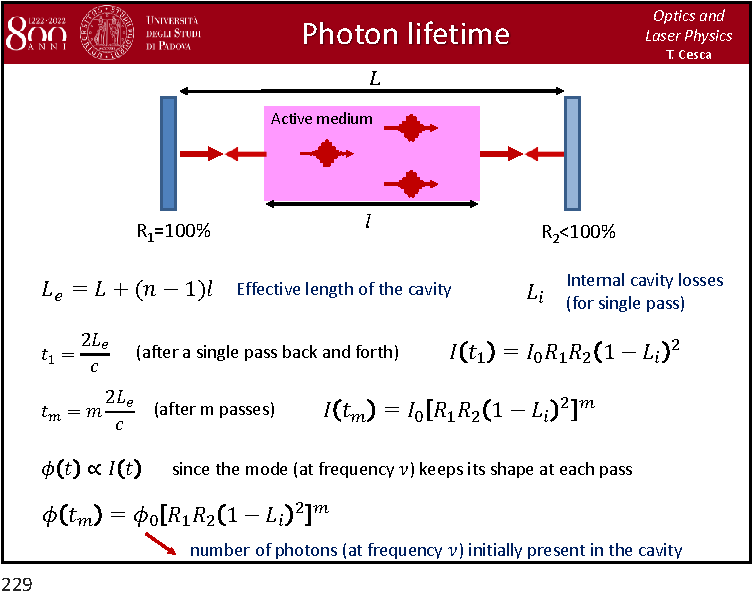
\includegraphics[page=1,width=1\textwidth]{../lessons/pdf_file/12_lecture.pdf}
\end{minipage}
\hspace{0.3cm}\vspace{0.3cm}
\begin{minipage}[c]{0.47\linewidth}

Longitudinal modes are sustained by the cavity and amplified by the active medium.

We want to determine the \textbf{lifetime} of a  \textbf{photon} which is related to the presence of losses inside the cavity.

Let us consider a Fabry-Perot cavity with two mirrors and with a length \( L \). The active medium is a solid state medium of size \( l \).

First, we compute the \textbf{effective length of the cavity} and we take into account of the losses by \( L_i \) the \textbf{internal cavity losses}.

Let us compute the time for a photon for pass back and forth trough the cavity.

We are not writing any term which is provided by the amplification of the active medium. We are just considering the effects of losses.

\end{minipage}

After \( m \) passes back and forth the time is \( t_m = m t_1 \). We can assume that the number of photon between the cavity is proportional to the intensity.  So, the temporal dependence of the intensity is proportional to the number of photons in the cavity.

\subsubsection*{Slide 2}

\begin{minipage}[]{0.5\linewidth}
\centering
\includegraphics[page=2,width=1\textwidth]{../lessons/pdf_file/12_lecture.pdf}
\end{minipage}
\hspace{0.3cm}\vspace{0.3cm}
\begin{minipage}[c]{0.47\linewidth}

We rewrite the number of photons in the camera as an exponential decay with constant given by the photon lifetime.

\end{minipage}

\subsubsection*{Slide 3}

\begin{minipage}[]{0.5\linewidth}
\centering
\includegraphics[page=3,width=1\textwidth]{../lessons/pdf_file/12_lecture.pdf}
\end{minipage}
\hspace{0.3cm}\vspace{0.3cm}
\begin{minipage}[c]{0.47\linewidth}

\( t_m \) are discrete values, but we can rewrite it in a continuous form.

\( \gamma   \) are the total logaritmic losses of the photon inside the cavity.

\end{minipage}

\newpage

\subsubsection*{Slide 4}

\begin{minipage}[]{0.5\linewidth}
\centering
\includegraphics[page=4,width=1\textwidth]{../lessons/pdf_file/12_lecture.pdf}
\end{minipage}
\hspace{0.3cm}\vspace{0.3cm}
\begin{minipage}[c]{0.47\linewidth}

These are some numbers to do some calculations.
So, typically photons survive within the cavity \( 150 \) ns.

\end{minipage}

\subsubsection*{Slide 5}

\begin{minipage}[]{0.5\linewidth}
\centering
\includegraphics[page=5,width=1\textwidth]{../lessons/pdf_file/12_lecture.pdf}
\end{minipage}
\hspace{0.3cm}\vspace{0.3cm}
\begin{minipage}[c]{0.47\linewidth}

Another parameter is the \textbf{cavity quality factor} and it is defined by the ratio of the energy of the mode at the frequency \( \nu  \) divided by the power dissipated by the cavity at that frequency.

The quality factor is directly proportional to the lifetime of photons.

\end{minipage}

\subsubsection*{Slide 6}

\begin{minipage}[]{0.5\linewidth}
\centering
\includegraphics[page=6,width=1\textwidth]{../lessons/pdf_file/12_lecture.pdf}
\end{minipage}
\hspace{0.3cm}\vspace{0.3cm}
\begin{minipage}[c]{0.47\linewidth}

As said, we can define the \textbf{bandwidth} of the modes. If you have a finite lifetime you have a finite bandwidth to consider.

\end{minipage}

\newpage

\subsubsection*{Slide 7}

\begin{minipage}[]{0.5\linewidth}
\centering
\includegraphics[page=7,width=1\textwidth]{../lessons/pdf_file/12_lecture.pdf}
\end{minipage}
\hspace{0.3cm}\vspace{0.3cm}
\begin{minipage}[c]{0.47\linewidth}

Just to have an idea about the numbers, we have \( Q sim 10^8\) which is extremely large. This means very narrow bandwidth.

\end{minipage}

\subsubsection*{Slide 8}

\begin{minipage}[]{0.5\linewidth}
\centering
\includegraphics[page=8,width=1\textwidth]{../lessons/pdf_file/12_lecture.pdf}
\end{minipage}
\hspace{0.3cm}\vspace{0.3cm}
\begin{minipage}[c]{0.47\linewidth}

Let us start describe the behavior of a laser in \textbf{continuous wave mode}.

We are adopting a phenomenological description with rate equations, not a description with quantum mechanics. It is a strong approach which in any cases provides most of the results.

We assume a \textbf{four-level laser} because they are the simplest system which can obtain laser action.

We will consider \textbf{single mode oscillation} (only one longitudinal mode with a given transverse profile).

We will assume that the active medium is \textbf{homogeneously broadened}: what is happening to an atom is happening to all the other atoms inside the active medium.

\end{minipage}

We have also \textbf{uniform energy density} of the mode on the active medium.
We are assuming the transverse profile of the mode is uniform in the perpendicular plane wrt to the cavity.

The final assumption is the \textbf{uniform pumping} at a \textbf{constant pumping rate} \( R_P \).

So, we study the CW behavior in a \textbf{space-independent rate equation} approach.
\subsubsection*{Slide 9}

\begin{minipage}[]{0.5\linewidth}
\centering
\includegraphics[page=9,width=1\textwidth]{../lessons/pdf_file/12_lecture.pdf}
\end{minipage}
\hspace{0.3cm}\vspace{0.3cm}
\begin{minipage}[c]{0.47\linewidth}

These are the rate equations.

The first one is about the number of photons in the 2 level.

The second is the one related to the number of photons inside the cavity.

\( V \) is the volume of the mode in the cavity.

Moreover, the \textbf{stimulated emission rate} can be written as a proportional function of the number of photons trough the factor \( B \).
Hence, we can rewrite the rate equations.

\( B \) is not the same of the Einstein's coefficient for stimulated emission \( B_{21} \)!

\( A_b \) is the \textbf{transverse section of the mode}.

\end{minipage}

\subsubsection*{Slide 10}

\begin{minipage}[]{0.5\linewidth}
\centering
\includegraphics[page=10,width=1\textwidth]{../lessons/pdf_file/12_lecture.pdf}
\end{minipage}
\hspace{0.3cm}\vspace{0.3cm}
\begin{minipage}[c]{0.47\linewidth}

\( t_t \) is the \textbf{transit time}, which correspond to the time for a photon to go from a mirror to the other.

We end up with a simplified expression for \( B \).

\end{minipage}

\subsubsection*{Slide 11}

\begin{minipage}[]{0.5\linewidth}
\centering
\includegraphics[page=11,width=1\textwidth]{../lessons/pdf_file/12_lecture.pdf}
\end{minipage}
\hspace{0.3cm}\vspace{0.3cm}
\begin{minipage}[c]{0.47\linewidth}

But \( W \) can be written also as a function of the Einstein's coefficient.

\end{minipage}

\subsubsection*{Slide 12}

\begin{minipage}[]{0.5\linewidth}
\centering
\includegraphics[page=12,width=1\textwidth]{../lessons/pdf_file/12_lecture.pdf}
\end{minipage}
\hspace{0.3cm}\vspace{0.3cm}
\begin{minipage}[c]{0.47\linewidth}

So, we have rewritten the rate equations in this way.

An important point to stress is that in the second equation the possibility that the number of photons increases as a consequence of spontaneous emission is not considered. Just stimulated emission is considered.
Instead, spontaneous emission was accounted in the first equation by the term \( -N_2/ \tau  \).

The reason why we are not considering any spontaneous emission term in the second equation is because we should consider only those photons that contribute to the given mode we are considering. It can be shown by quantum mechanics that the rate equation is this equation and to consider an extra photon to take into account spontaneous emission.
However, we consider a very huge number of photons when the laser is active, so this extra photon can be neglected.

\end{minipage}

In order to have laser action starting, we will consider to have at least one photon in the cavity and it is produced by spontaneous emission. So, we will consider \textbf{spontaneous emission as a trigger for laser action}.

\subsubsection*{Slide 13}

\begin{minipage}[]{0.5\linewidth}
\centering
\includegraphics[page=13,width=1\textwidth]{../lessons/pdf_file/12_lecture.pdf}
\end{minipage}
\hspace{0.3cm}\vspace{0.3cm}
\begin{minipage}[c]{0.47\linewidth}

Since we are dealing with a four-level system, the \textbf{population inversion} is equal to \( N_2 \). So, we can rewrite the rate equations in terms of number of photon inside the cavity.

The term \( \Phi / \tau_c \) is due to the lifetime, so due to the fact that we have losses inside the cavity. The last term is the number of photon per unit of time which are lost from the cavity due to the fact they are extracted from the cavity to produce the laser beam.

\end{minipage}

\subsubsection*{Slide 14}

\begin{minipage}[]{0.5\linewidth}
\centering
\includegraphics[page=14,width=1\textwidth]{../lessons/pdf_file/12_lecture.pdf}
\end{minipage}
\hspace{0.3cm}\vspace{0.3cm}
\begin{minipage}[c]{0.47\linewidth}

We can immediately calculate the \textbf{power of the beam}: the number of photon per unit of time that we are extracting from the cavity multiplied by the energy of those photons. The output beam is produced by those photons that are extracted from the cavity due to the outcoupling from the outcoupler mirror.

\end{minipage}

\subsubsection*{Slide 15}

\begin{minipage}[]{0.5\linewidth}
\centering
\includegraphics[page=15,width=1\textwidth]{../lessons/pdf_file/12_lecture.pdf}
\end{minipage}
\hspace{0.3cm}\vspace{0.3cm}
\begin{minipage}[c]{0.47\linewidth}

Just for this low power level you can gate a number of photons which is very large.

\end{minipage}

\subsubsection*{Slide 16}

\begin{minipage}[]{0.5\linewidth}
\centering
\includegraphics[page=16,width=1\textwidth]{../lessons/pdf_file/12_lecture.pdf}
\end{minipage}
\hspace{0.3cm}\vspace{0.3cm}
\begin{minipage}[c]{0.47\linewidth}

This is another example.

\end{minipage}



\end{document}
